\documentclass{article}
\usepackage{physics}
\usepackage{graphicx}
\usepackage{caption}
\usepackage{amsmath}
\usepackage{bm}
\usepackage{framed}
\usepackage{authblk}
\usepackage{empheq}
\usepackage{amsfonts}
\usepackage{esint}
\usepackage[makeroom]{cancel}
\usepackage{dsfont}
\usepackage{centernot}
\usepackage{mathtools}
\usepackage{bigints}
\usepackage{amsthm}
\theoremstyle{definition}
\newtheorem{lemma}{Lemma}
\newtheorem{defn}{Definition}[section]
\newtheorem{prop}{Proposition}[section]
\newtheorem{rmk}{Remark}[section]
\newtheorem{thm}{Theorem}[section]
\newtheorem{exmp}{Example}[section]
\newtheorem{prob}{Problem}[section]
\newtheorem{sln}{Solution}[section]
\newtheorem*{prob*}{Problem}
\newtheorem{exer}{Exercise}[section]
\newtheorem*{exer*}{Exercise}
\newtheorem*{sln*}{Solution}
\usepackage{empheq}
\usepackage{tensor}
\usepackage{xcolor}
%\definecolor{colby}{rgb}{0.0, 0.0, 0.5}
\definecolor{MIT}{RGB}{163, 31, 52}
\usepackage[pdftex]{hyperref}
%\hypersetup{colorlinks,urlcolor=colby}
\hypersetup{colorlinks,linkcolor={MIT},citecolor={MIT},urlcolor={MIT}}  
\usepackage[left=1in,right=1in,top=1in,bottom=1in]{geometry}

\usepackage{newpxtext,newpxmath}
\newcommand*\widefbox[1]{\fbox{\hspace{2em}#1\hspace{2em}}}

\newcommand{\p}{\partial}
\newcommand{\R}{\mathbb{R}}
\newcommand{\C}{\mathbb{C}}
\newcommand{\lag}{\mathcal{L}}
\newcommand{\nn}{\nonumber}
\newcommand{\ham}{\mathcal{H}}
\newcommand{\M}{\mathcal{M}}
\newcommand{\I}{\mathcal{I}}
\newcommand{\K}{\mathcal{K}}
\newcommand{\F}{\mathcal{F}}
\newcommand{\w}{\omega}
\newcommand{\lam}{\lambda}
\newcommand{\al}{\alpha}
\newcommand{\be}{\beta}
\newcommand{\x}{\xi}

\newcommand{\G}{\mathcal{G}}

\newcommand{\f}[2]{\frac{#1}{#2}}

\newcommand{\ift}{\infty}

\newcommand{\lp}{\left(}
\newcommand{\rp}{\right)}

\newcommand{\lb}{\left[}
\newcommand{\rb}{\right]}

\newcommand{\lc}{\left\{}
\newcommand{\rc}{\right\}}


\newcommand{\V}{\mathbf{V}}
\newcommand{\U}{\mathcal{U}}
\newcommand{\Id}{\mathcal{I}}
\newcommand{\D}{\mathcal{D}}
\newcommand{\Z}{\mathcal{Z}}

%\setcounter{chapter}{-1}


\usepackage{enumitem}



\usepackage{subfig}
\usepackage{listings}
\captionsetup[lstlisting]{margin=0cm,format=hang,font=small,format=plain,labelfont={bf,up},textfont={it}}
\renewcommand*{\lstlistingname}{Code \textcolor{violet}{\textsl{Mathematica}}}
\definecolor{gris245}{RGB}{245,245,245}
\definecolor{olive}{RGB}{50,140,50}
\definecolor{brun}{RGB}{175,100,80}

%\hypersetup{colorlinks,urlcolor=colby}
\lstset{
	tabsize=4,
	frame=single,
	language=mathematica,
	basicstyle=\scriptsize\ttfamily,
	keywordstyle=\color{black},
	backgroundcolor=\color{gris245},
	commentstyle=\color{gray},
	showstringspaces=false,
	emph={
		r1,
		r2,
		epsilon,epsilon_,
		Newton,Newton_
	},emphstyle={\color{olive}},
	emph={[2]
		L,
		CouleurCourbe,
		PotentielEffectif,
		IdCourbe,
		Courbe
	},emphstyle={[2]\color{blue}},
	emph={[3]r,r_,n,n_},emphstyle={[3]\color{magenta}}
}






\begin{document}
\begin{framed}
\noindent Name: \textbf{Huan Q. Bui}\\
Course: \textbf{8.321 - Quantum Theory I}\\
Problem set: \textbf{\#3}
\end{framed}
	




\noindent \textbf{1. }
\begin{equation*}
A = \begin{pmatrix}
1 & 0 & 1\\
0 & 0 & 0\\
1 & 0 & 1
\end{pmatrix} 
\quad\quad \quad 
B = \begin{pmatrix}
2 & 1 & 1 \\
1 & 0 & -1\\
1 & -1 & 2
\end{pmatrix}.
\end{equation*}

\begin{enumerate}[label=(\alph*)]
	\item To show that $AB$ commute, we simply compute their commutator:
	\begin{align*}
	[A,B] = \begin{pmatrix}
	1 & 0 & 1\\
	0 & 0 & 0\\
	1 & 0 & 1
	\end{pmatrix} 
	\begin{pmatrix}
	2 & 1 & 1 \\
	1 & 0 & -1\\
	1 & -1 & 2
	\end{pmatrix}
	- 
	\begin{pmatrix}
	2 & 1 & 1 \\
	1 & 0 & -1\\
	1 & -1 & 2
	\end{pmatrix}
	\begin{pmatrix}
	1 & 0 & 1\\
	0 & 0 & 0\\
	1 & 0 & 1
	\end{pmatrix} 
	= 
	\begin{pmatrix}
	3 & 0 & 3\\
	0 & 0 & 0\\
	3 & 0 & 3
	\end{pmatrix}
	-
	\begin{pmatrix}
	3 & 0 & 3\\
	0 & 0 & 0\\
	3 & 0 & 3
	\end{pmatrix} = 
	\begin{pmatrix}
	0 & 0 & 0\\
	0 & 0 & 0\\
	0 & 0 & 0
	\end{pmatrix}.   
	\end{align*}
	So, $A$ and $B$ commute.
	
	
	\item Notice that $\rank(A) = 1$. So $A$ must have eigenvalue of zero with multiplicity of two. The other eigenvalue is $2$ by inspection, where the corresponding eigenvector is $(1,0,1)^\top$. The other two $0$-eigenvectors must span the subspace orthogonal to $(1,0,1)^\top$. We may choose $(0,1,0)^\top$ and $(-1,0,1)^\top$.\\
	
	To find the eigenvalues of $B$ we may use the traditional method of characteristic polynomials. 
	\begin{align*}
	0 = \det(B-\lambda \mathbb{I}) = -6-\lambda +4 \lambda^2 - \lambda^3 \implies 0 = (\lambda-3)(\lambda-2)(\lambda+1).
	\end{align*}
	The corresponding eigenvectors are
	\begin{align*}
	&\begin{pmatrix}
	2 & 1 & 1 \\
	1 & 0 & -1\\
	1 & -1 & 2
	\end{pmatrix}\vec{x}_1 = 3\vec{x}_1 \implies \vec{x}_1 = \begin{pmatrix}
	1 \\ 0 \\ 1
	\end{pmatrix}\\
	&\begin{pmatrix}
	2 & 1 & 1 \\
	1 & 0 & -1\\
	1 & -1 & 2
	\end{pmatrix}\vec{x}_2 = 2\vec{x}_2 \implies \vec{x}_2 = \begin{pmatrix}
	-1 \\ -1 \\ 1
	\end{pmatrix}\\
	&\begin{pmatrix}
	2 & 1 & 1 \\
	1 & 0 & -1\\
	1 & -1 & 2
	\end{pmatrix}\vec{x}_3 = -1\vec{x}_3 \implies \vec{x}_3 = \begin{pmatrix}
	-1 \\ 2 \\ 1
	\end{pmatrix}
	\end{align*}
	
	
	\item It is clear that $(1,0,1)^\top$ is a simultaneous eigenvector of $A$ and $B$. Also notice that the eigenvectors $\vec{x}_2$ and $\vec{x}_3$ of $B$ are orthogonal to each other and to $(1,0,1)^\top$. This means $\vec{x}_2$ and $\vec{x}_3$ span the subspace associated with the eigenvalue zero for $A$. Thus, $\vec{x}_2$, $\vec{x}_3$ are eigenvectors of $A$ and it suffices to normalize $\vec{x}_1, \vec{x}_2, \vec{x}_3$ to form a unitary matrix:
	\begin{align*}
	\boxed{U = \begin{pmatrix}
	1/\sqrt{2}  & -1/\sqrt{3} & -1/\sqrt{6}  \\
	0 & -1/\sqrt{3} & 2/\sqrt{6}   \\
	1 /\sqrt{2} & 1/\sqrt{3} & 1/\sqrt{6} 	
	\end{pmatrix}}
	\end{align*} 
	Simultaneous diagonalization of $A$ and $B$:
	\begin{align*}
	&U^\dagger A U = \begin{pmatrix}
	2 & 0 & 0 \\
	0&0&0\\
	0&0&0
	\end{pmatrix}\\
	&U^\dagger B U = \begin{pmatrix}
	3 & 0 & 0 \\
	0 & 2 & 0 \\ 
	0 & 0 & -1
	\end{pmatrix}
	\end{align*}
	as desired.
\end{enumerate}



\noindent \textbf{2. } $N$ spin-$1/2$ particles in 
\begin{align*}
\ham = \ham_2^{(1)} \otimes \ham_2^{(2)} \otimes \dots \otimes \ham_2^{(n)}.
\end{align*}
where each $\ham_2^{(i)}$ is two-dimensional.


\begin{enumerate}[label=(\alph*)]
	\item The dimension of $\ham$ is $2^n$.
	
	\item $S_z = S_z^{(1)} + S_z^{(2)} + \dots + S_z^{(n)}$. There are ${n\choose i}$ product (eigen)states with $i$ particles in $\ket{\uparrow}$ and $(n-i)$ particles in $\ket{\downarrow}$. For the product state with $i$ particles in $\ket{\uparrow}$, the corresponding eigenvalue is 
	\begin{align*}
	\lambda = \f{\hbar}{2}i - \f{\hbar}{2}(n-i) = \f{\hbar}{2}\lp 2i-n \rp,\quad\quad i = 0,1,2,\dots,n
	\end{align*}
	So, the spectrum of $S_z$ is 
	\begin{align*}
	\sigma(S_z) = \lc \f{n\hbar}{2}, \f{(n-2)\hbar}{2},\dots, \f{-(n-2)\hbar}{2}, \f{-n\hbar}{2}   \rc
	\end{align*}
	There are $n+1$ distinct eigenvalues. The multiplicity of each $\lambda_i$ is ${n\choose{i}}$ where $\lambda_i$ is the eigenvalue associated with the product state with $i$ spins in $\ket{\uparrow}$. \\
	
	As a sanity check, the sum of the multiplicities must be $2^n$. This is the case here due to a well-known combinatorial relation:
	\begin{align*}
	\sum_{i=0}^n {n\choose{i}} = (1+1)^n = 2^n.
	\end{align*}
	
	\item $I = \mathbf{S}^{(1)}\cdot \mathbf{S}^{(2)}+ \mathbf{S}^{(2)}\cdot \mathbf{S}^{(3)} + \dots + \mathbf{S}^{(N-1)}\cdot \mathbf{S}^{(N)}+ \mathbf{S}^{(N)}\cdot \mathbf{S}^{(1)}$. We claim that $[I,S_z] = 0$ and shall prove this by induction. Consider the base case where $N=2$. We may prove it directly by calculating the Kronecker product of the Pauli matrices (working in the $z$-basis).
	\begin{align*}
	&I = \mathbf{S}^{(1)} \cdot \mathbf{S}^{(2)} + \mathbf{S}^{(2)}\cdot \mathbf{S}^{(1)} = 2\lb S_x^{(1)}\otimes S_x^{(2)} + S_y^{(1)} \otimes S_y^{(2)} + S_z^{(1)}\otimes S_z^{(2)}  \rb\\
	&S_z = S_z^{(1)} \otimes \mathbb{I} + \mathbb{I}\otimes S_z^{(2)}.
	\end{align*}
	In Mathematica:
	\begin{lstlisting}
	In[2]:= X = PauliMatrix[1];
	
	In[3]:= Y = PauliMatrix[2];
	
	In[4]:= Z = PauliMatrix[3];
	
	In[6]:= Id = IdentityMatrix[2];
	
	In[8]:= II = 
	2*(KroneckerProduct[X, X] + KroneckerProduct[Y, Y] + 
	KroneckerProduct[Z, Z]);
	
	In[9]:= SZ = KroneckerProduct[Z, Id] + KroneckerProduct[Id, Z];
	
	In[12]:= Commutator = II . SZ - SZ . II;
	
	In[13]:= Commutator
	
	Out[13]= {{0, 0, 0, 0}, {0, 0, 0, 0}, {0, 0, 0, 0}, {0, 0, 0, 0}}
	\end{lstlisting}
	Thus 
	\begin{align*}
	[I^{(2)}, Sz]  = 0.
	\end{align*}
	Now let us assume that $[I, S_z]$ is true up to $N$. We will show that $[I,S_z]$ also holds for $N+1$. This is a straightforward computation. Let us call $I = I_N + I'$ where 
	\begin{align*}
	I_N 
	&= \mathbf{S}^{(1)}\cdot \mathbf{S}^{(2)}+ \mathbf{S}^{(2)}\cdot \mathbf{S}^{(3)} + \dots + \mathbf{S}^{(N-1)}\cdot \mathbf{S}^{(N)}+ \mathbf{S}^{(N)}\cdot \mathbf{S}^{(1)} 
	\end{align*}
	and 
	\begin{align*}
	I' = \mathbf{S}^{(N)}\cdot \mathbf{S}^{(N+1)} + \mathbf{S}^{(N+1)}\cdot \mathbf{S}^{(1)}  -\mathbf{S}^{(N)}\cdot \mathbf{S}^{(1)} 
	\end{align*}
	Moreover, let us write 
	\begin{align*}
	S_z = S_z^{(N+1)} +\sum_{i=1}^N S_z^{(i)}.
	\end{align*}
	Since $I_N$ commute with both $S_z^{N+1}$ (by the fact that $S_z^{N+1}$ does not act on the spins $i=1,\dots,N$) and $\sum_i^N S_z^{(i)}$ (by inductive hypothesis), we have
	\begin{align*}
	[I,S_z]
	&= \lb I_N + I' , S_z^{(N+1)} +\sum_{i=1}^N S_z^{(i)} \rb \\
	&= \lb I' , S_z^{(N+1)}\rb  +\lb I', \sum_{i=1}^N S_z^{(i)} \rb \\
	&= \lb \mathbf{S}^{(N)}\cdot \mathbf{S}^{(N+1)} + \mathbf{S}^{(N+1)}\cdot \mathbf{S}^{(1)} , S_z^{(N+1)} \rb + \lb \mathbf{S}^{(N)}\cdot \mathbf{S}^{(N+1)} + \mathbf{S}^{(N+1)}\cdot \mathbf{S}^{(1)}  , \sum_{i=1}^N S_z^{(i)}\rb 
	\end{align*}
	where we have used the following facts: 
	\begin{align*}
	&\lb  \mathbf{S}^{(N)}\cdot \mathbf{S}^{(1)} , S_z^{(N+1)} \rb = 0\\
	&\lb \mathbf{S}^{(N)}\cdot \mathbf{S}^{(1)} ,  \sum_{i=1}^N S_z^{(i)} \rb = \lb \mathbf{S}^{(N)}\cdot \mathbf{S}^{(1)}, S_z^{(1)} + S_z^{(N)} \rb = 0
	\end{align*}
	where the second comes from the $N=2$ result. We may simplify $[I,S_z]$ even further:
	\begin{align*}
	[I,S_z] 
	&=  \lb \mathbf{S}^{(N)}\cdot \mathbf{S}^{(N+1)} + \mathbf{S}^{(N+1)}\cdot \mathbf{S}^{(1)} , S_z^{(N+1)} \rb + \lb \mathbf{S}^{(N)}\cdot \mathbf{S}^{(N+1)} + \mathbf{S}^{(N+1)}\cdot \mathbf{S}^{(1)}  , S_z^{(1)} + S_z^{(N)}\rb \\
	&= \lb \mathbf{S}^{(N)}\cdot \mathbf{S}^{(N+1)} + \mathbf{S}^{(N+1)}\cdot \mathbf{S}^{(1)} , S_z^{(1)} + S_z^{(N)} + S_z^{(N+1)} \rb\\
	&= \lb \mathbf{S}^{(N)}\cdot \mathbf{S}^{(N+1)}, S_z^{(1)} + S_z^{(N)} + S_z^{(N+1)} \rb + \lb  \mathbf{S}^{(N+1)}\cdot \mathbf{S}^{(1)} ,  S_z^{(1)} + S_z^{(N)} + S_z^{(N+1)}\rb \\
	&= \lb \mathbf{S}^{(N)}\cdot \mathbf{S}^{(N+1)}, S_z^{(N)} + S_z^{(N+1)} \rb + \lb  \mathbf{S}^{(N+1)}\cdot \mathbf{S}^{(1)} ,  S_z^{(1)}  + S_z^{(N+1)}\rb\\
	&= 0 + 0 \\
	&=0 
	\end{align*}
	in view of the $N=2$ base case. We thus conclude that $I$ and $S_z$ are compatible observables.
	 
	
	
	\item Spectrum and degeneracies of $I$ for $N=2,3,4$. 
	\begin{itemize}
		\item $N=2$ (dropping the factor of $\hbar^2/4$ for clarity):
		\begin{align*}
		\boxed{\sigma(I_2) =  \{ -6, \underbrace{2}_{\text{deg.}=3}  \} }
		\end{align*}
		\item $N=3$ (dropping the factor of $\hbar^2/4$ for clarity):
		\begin{align*}
		\boxed{\sigma(I_3) = \{ \underbrace{-3}_{\text{deg.}=4}, \underbrace{3}_{\text{deg.}=4}  \}} 
		\end{align*}
		\item $N=4$ (dropping the factor of $\hbar^2/4$ for clarity):
		\begin{align*}
		\boxed{\sigma(I_4) = \{ -8, \underbrace{-4}_{\text{deg.}=3}, \underbrace{4}_{\text{deg.}=5}, \underbrace{0}_{\text{deg.}=7}  \} }
		\end{align*}
	\end{itemize}
	For this problem I have used a brute force via a simple routine in MATLAB which allows me compute the spectrum for large $N$'s. Below is the code. 
	\begin{lstlisting}
	N    = 10;
	state0 = zeros(2^N,1);
	eigv = 0;
	
	Sz = [1 0 ; 0 -1];
	Sx = [0 1 ; 1 0];
	Sy = [0 -complex(0,1); complex(0,1) 0];
	Id = [1 0 ; 0 1];
	
	% ZZ, YY, XX
	cell_ZZ = cell(N,1);
	cell_YY = cell(N,1);
	cell_XX = cell(N,1);
	termZ = zeros(2,2);
	termY = zeros(2,2);
	termX = zeros(2,2);
	operatorsZ = cell(N,1);
	operatorsY = cell(N,1);
	operatorsX = cell(N,1);
	
	for n = 0:N-2
	operatorsZ = horzcat( horzcat( repmat({Id},1,n)  ,horzcat({Sz}, {Sz})), repmat({Id}, 1 , N-2-n));
	operatorsY = horzcat( horzcat( repmat({Id},1,n)  ,horzcat({Sy}, {Sy})), repmat({Id}, 1 , N-2-n));
	operatorsX = horzcat( horzcat( repmat({Id},1,n)  ,horzcat({Sx}, {Sx})), repmat({Id}, 1 , N-2-n));
	termZ = operatorsZ{1};
	termY = operatorsY{1};
	termX = operatorsX{1};
	for o = 2:N 
	termZ = kron(termZ, operatorsZ{o});
	termY = kron(termY, operatorsY{o});
	termX = kron(termX, operatorsX{o});
	end
	cell_ZZ{n+1} = termZ;
	cell_YY{n+1} = termY;
	cell_XX{n+1} = termX;
	end
	
	
	% deals with the periodic term
	operatorsZ = horzcat(horzcat( {Sz}, repmat({Id}, 1, N-2) ), {Sz} );
	operatorsY = horzcat(horzcat( {Sy}, repmat({Id}, 1, N-2) ), {Sy} );
	operatorsX = horzcat(horzcat( {Sx}, repmat({Id}, 1, N-2) ), {Sx} );
	termZ = operatorsZ{1};
	termY = operatorsY{1};
	termX = operatorsX{1};
	for o = 2:N 
	termZ = kron(termZ, operatorsZ{o});
	termY = kron(termY, operatorsY{o});
	termX = kron(termX, operatorsX{o});
	end
	cell_ZZ{N} = termZ;
	cell_YY{N} = termY;
	cell_XX{N} = termX;
	
	% generates Hamiltonian
	Hamiltonian = zeros(2^N,2^N);
	for i = 1:N
	Hamiltonian = Hamiltonian + cell_ZZ{i} + cell_XX{i} + cell_YY{i};
	end
	
	
	[state0, eigv] = eig(Hamiltonian);
	
	disp(transpose(diag(eigv)));
	disp(state0);
	\end{lstlisting}
	
	
	
	\item By running the MATLAB program for a range of $N$'s, we find that
	\begin{align*}
	\boxed{\lambda_\text{max}^{(N)} = N} \quad\quad\text{restoring } \hbar^2/4 \implies \lambda_\text{max}^{(N)} = N\hbar^2/4
	\end{align*}
	with degeneracy $N+1$. Since the degenaracy grows linearly in $N$, we have multiple choices for an eigenvector associated with each of these eigenvalues. However, using MATLAB we may find that the eigenvectors
	\begin{align*}
	\boxed{\ket{\psi} = (0,0,\dots, 1)^\top \quad\quad \text{and} \quad\quad \ket{\phi} = (1,0,\dots,0)^\top} 
	\end{align*}
	are always associated with the largest positive eigenvalue. 
	
	\item The largest $N$ I could compute in a reasonable amount of time (\textbf{48 seconds}) is $\boxed{N=22}$
	\begin{figure}[!htb]
		\centering
		\includegraphics[width=0.75\textwidth]{2f.eps}
	\end{figure} 
	We see that $\lambda{\text{min}}^{(N)}$ also decreases without bounds and appears to scale linearly in $N$ for small $N$, similar to $\lambda_\text{max}^{(N)}$. I did a linear fit to the data and found that 
	\begin{align*}
	\lambda_\text{min}^{(N)} \approx \f{\hbar^2}{4}\lp -1.7684N + 0.055027\rp .
	\end{align*} 
	A few associated eigenvectors can also be found using the previous MATLAB routine, \textcolor{blue}{but I can't seem to find anything special about these eigenvectors in relation to $N$.}\\
	
	
	
	
	
	MATLAB code (optimized for the minimum eigenvalue problem):
	\begin{lstlisting}
	clear 
	%%%%%%%%%%%%%%%%%%%
	% clock starts
	tic 
	% clock starts
	%%%%%%%%%%%%%%%%%%%
	
	N = 22;
	parfor j=1:N-1
	data(j) = MinEig(j+1);
	end
	plot(2:1:N, data, 'LineWidth',2)
	ylabel('Smallest Eigenvalue')
	xlabel('N')
	grid on
	
	% linear fit
	p = polyfit(2:1:N, data, 1);
	fit = polyval(p,2:1:N);
	hold on
	plot(2:1:N,fit, 'LineWidth', 1)
	hold off
	
	% display fit eqn in legend
	a = p(1);
	b = p(2);
	legend('calculated', ['fit: minEig = ' num2str(a) 'N + ' num2str(b)])
	
	
	
	%%%%%%%%%%%%%%%%%%%
	% clock ends
	Duration = seconds(round(toc));
	Duration.Format = 'hh:mm:ss';
	disp(['Time taken : ' char(Duration)]);
	% disp(['Time in sec: ' num2str(toc)]);
	disp(' ')
	% clock ends
	%%%%%%%%%%%%%%%%%%%
	
	% returns the smallest eigenvalue
	function minEig = MinEig(N)
	
	Sz = sparse([1 0 ; 0 -1]);
	Sx = sparse([0 1 ; 1 0]);
	Sy = sparse([0 -complex(0,1); complex(0,1) 0]);
	Id = sparse([1 0 ; 0 1]);
	
	% ZZ, YY, XX
	cell_ZZ = cell(N,1);
	cell_YY = cell(N,1);
	cell_XX = cell(N,1);
	termZ = zeros(2,2);
	termY = zeros(2,2);
	termX = zeros(2,2);
	operatorsZ = cell(N,1);
	operatorsY = cell(N,1);
	operatorsX = cell(N,1);
	
	parfor n = 0:N-2
	operatorsZ = horzcat( horzcat( repmat({Id},1,n)  ,horzcat({Sz}, {Sz})), repmat({Id}, 1 , N-2-n));
	operatorsY = horzcat( horzcat( repmat({Id},1,n)  ,horzcat({Sy}, {Sy})), repmat({Id}, 1 , N-2-n));
	operatorsX = horzcat( horzcat( repmat({Id},1,n)  ,horzcat({Sx}, {Sx})), repmat({Id}, 1 , N-2-n));
	termZ = operatorsZ{1};
	termY = operatorsY{1};
	termX = operatorsX{1};
	for o = 2:N
	termZ = sparse(kron(termZ, operatorsZ{o}));
	termY = sparse(kron(termY, operatorsY{o}));
	termX = sparse(kron(termX, operatorsX{o}));
	end
	cell_ZZ{n+1} = termZ;
	cell_YY{n+1} = termY;
	cell_XX{n+1} = termX;
	end
	
	% periodic term
	operatorsZ = horzcat(horzcat( {Sz}, repmat({Id}, 1, N-2) ), {Sz} );
	operatorsY = horzcat(horzcat( {Sy}, repmat({Id}, 1, N-2) ), {Sy} );
	operatorsX = horzcat(horzcat( {Sx}, repmat({Id}, 1, N-2) ), {Sx} );
	termZ = operatorsZ{1};
	termY = operatorsY{1};
	termX = operatorsX{1};
	for o = 2:N
	termZ = sparse(kron(termZ, operatorsZ{o}));
	termY = sparse(kron(termY, operatorsY{o}));
	termX = sparse(kron(termX, operatorsX{o}));
	end
	cell_ZZ{N} = termZ;
	cell_YY{N} = termY;
	cell_XX{N} = termX;
	
	% generates Hamiltonian
	Hamiltonian = sparse(2^N,2^N);
	parfor i = 1:N
	Hamiltonian = Hamiltonian + cell_ZZ{i} + cell_XX{i} + cell_YY{i};
	end
	% exact diagonalization
	eigv = eigs(Hamiltonian,1,'smallestreal');
	
	% returns smallest eigenvalue
	minEig = eigv;
	
	end
	\end{lstlisting}
	
	\item We have 
	\begin{align*}
	\ham  = bx S_z -a(1-x)I.
	\end{align*}
	With $b = a\hbar$, we may set $a=1$ and $\hbar=1$, so that 
	\begin{align*}
	\ham = \f{x}{2}S_z - \f{(1-x)}{4}I
	\end{align*}
	where we have nondimensionalized $S_z\propto \hbar/2$ and $I \propto \hbar^2/4$. We can also multiply $\ham$ by $4$ to remove all denominators:
	\begin{align*}
	\ham = 2xS_z - (1-x)I.
	\end{align*}
	
	\begin{figure}[!htb]
		\centering
		\begin{minipage}{0.49\textwidth}
			\includegraphics[width=\textwidth]{2g.eps}
		\end{minipage}
		\begin{minipage}{0.49\textwidth}
			\includegraphics[width=\textwidth]{2g_N3.eps}
		\end{minipage}
		\begin{minipage}{0.49\textwidth}
			\includegraphics[width=\textwidth]{2g_N4.eps}
		\end{minipage}
	\end{figure}

	The figures generated using the MATLAB code below show good agreement with what we found in the previous parts (setting $x=0$ and flipping the signs of the spectrum gives the results of Part (d)). When $x=1$, the spectra of $H$ are twice what we found in Part (b), which can be explained by the extra leading factor of $2$ on $S_z$ in the Hamiltonian, but are otherwise consistent. For example, at $x=1$ and $N=3$ we find $4=3+1$ distinct eigenvalues. To count degeneracies requires looking at the spectra numerically, since some of the splittings in the figures overlap. But in any case, the degeneracies are also consistent with what we found in Part (b). 
	\begin{lstlisting}
	clear crc
	clear all
	
	N = 4;
	res = 400;
	x = 0:1/res:1-1/res;
	figure(1)
	for j=0:1:res-1
	eigv = Bfield(N,j/res); 
	hold on
	X = (j/res)*ones(2^N,1);
	plot(X,eigv,'Marker','o', 'MarkerSize', 2, 'Color', 'r', 'LineStyle', 'None')
	hold off
	end
	hold off
	grid on
	
	xlabel('x')
	ylabel('Eigenvalues')
	title(['Spectrum of H for N=' num2str(N)])
	
	
	
	
	function eigv = Bfield(N,x)
	Sz = [1 0 ; 0 -1];
	Sx = [0 1 ; 1 0];
	Sy = [0 -complex(0,1); complex(0,1) 0];
	Id = [1 0 ; 0 1];
	
	% ZZ, YY, XX
	cell_ZZ = cell(N,1);
	cell_YY = cell(N,1);
	cell_XX = cell(N,1);
	termZ = zeros(2,2);
	termY = zeros(2,2);
	termX = zeros(2,2);
	operatorsZ = cell(N,1);
	operatorsY = cell(N,1);
	operatorsX = cell(N,1);
	
	for n = 0:N-2
	operatorsZ = horzcat( horzcat( repmat({Id},1,n)  ,horzcat({Sz}, {Sz})), repmat({Id}, 1 , N-2-n));
	operatorsY = horzcat( horzcat( repmat({Id},1,n)  ,horzcat({Sy}, {Sy})), repmat({Id}, 1 , N-2-n));
	operatorsX = horzcat( horzcat( repmat({Id},1,n)  ,horzcat({Sx}, {Sx})), repmat({Id}, 1 , N-2-n));
	termZ = operatorsZ{1};
	termY = operatorsY{1};
	termX = operatorsX{1};
	for o = 2:N 
	termZ = kron(termZ, operatorsZ{o});
	termY = kron(termY, operatorsY{o});
	termX = kron(termX, operatorsX{o});
	end
	cell_ZZ{n+1} = termZ;
	cell_YY{n+1} = termY;
	cell_XX{n+1} = termX;
	end
	
	
	% deals with the periodic term
	operatorsZ = horzcat(horzcat( {Sz}, repmat({Id}, 1, N-2) ), {Sz} );
	operatorsY = horzcat(horzcat( {Sy}, repmat({Id}, 1, N-2) ), {Sy} );
	operatorsX = horzcat(horzcat( {Sx}, repmat({Id}, 1, N-2) ), {Sx} );
	termZ = operatorsZ{1};
	termY = operatorsY{1};
	termX = operatorsX{1};
	for o = 2:N 
	termZ = kron(termZ, operatorsZ{o});
	termY = kron(termY, operatorsY{o});
	termX = kron(termX, operatorsX{o});
	end
	cell_ZZ{N} = termZ;
	cell_YY{N} = termY;
	cell_XX{N} = termX;
	
	
	% generates Sz
	% generate the fZ cell array of the Hamiltonian:
	term = sparse(2,2);
	cell_fZ = cell(N,1);
	operators = cell(N,1);
	for n = 0:N-1
	operators = horzcat( horzcat( repmat({Id},1,n), {Sz}), repmat({Id}, 1 , N-1-n));
	term = operators{1};
	for o = 2:N 
	term = sparse(kron(term, operators{o}));
	end
	cell_fZ{n+1} = term;
	end
	
	% generates Hamiltonian
	Hamiltonian = zeros(2^N,2^N);
	for i = 1:N
	Hamiltonian = Hamiltonian + 2*x*cell_fZ{i} - (1-x)*(cell_ZZ{i} + cell_XX{i} + cell_YY{i});
	end
	
	eigv = eig(Hamiltonian);
	
	end

	\end{lstlisting}
\end{enumerate}






\noindent \textbf{3. Qubits}



\begin{enumerate}[label=(\alph*)]
	\item 
	
	\item 
	
	
	\item
	
	
	\item 
	
	
	\item 
\end{enumerate}




	
\end{document}








